
% Default to the notebook output style

    


% Inherit from the specified cell style.




    
\documentclass[11pt]{article}

    
    
    \usepackage[T1]{fontenc}
    % Nicer default font (+ math font) than Computer Modern for most use cases
    \usepackage{mathpazo}

    % Basic figure setup, for now with no caption control since it's done
    % automatically by Pandoc (which extracts ![](path) syntax from Markdown).
    \usepackage{graphicx}
    % We will generate all images so they have a width \maxwidth. This means
    % that they will get their normal width if they fit onto the page, but
    % are scaled down if they would overflow the margins.
    \makeatletter
    \def\maxwidth{\ifdim\Gin@nat@width>\linewidth\linewidth
    \else\Gin@nat@width\fi}
    \makeatother
    \let\Oldincludegraphics\includegraphics
    % Set max figure width to be 80% of text width, for now hardcoded.
    \renewcommand{\includegraphics}[1]{\Oldincludegraphics[width=.8\maxwidth]{#1}}
    % Ensure that by default, figures have no caption (until we provide a
    % proper Figure object with a Caption API and a way to capture that
    % in the conversion process - todo).
    \usepackage{caption}
    \DeclareCaptionLabelFormat{nolabel}{}
    \captionsetup{labelformat=nolabel}

    \usepackage{adjustbox} % Used to constrain images to a maximum size 
    \usepackage{xcolor} % Allow colors to be defined
    \usepackage{enumerate} % Needed for markdown enumerations to work
    \usepackage{geometry} % Used to adjust the document margins
    \usepackage{amsmath} % Equations
    \usepackage{amssymb} % Equations
    \usepackage{textcomp} % defines textquotesingle
    % Hack from http://tex.stackexchange.com/a/47451/13684:
    \AtBeginDocument{%
        \def\PYZsq{\textquotesingle}% Upright quotes in Pygmentized code
    }
    \usepackage{upquote} % Upright quotes for verbatim code
    \usepackage{eurosym} % defines \euro
    \usepackage[mathletters]{ucs} % Extended unicode (utf-8) support
    \usepackage[utf8x]{inputenc} % Allow utf-8 characters in the tex document
    \usepackage{fancyvrb} % verbatim replacement that allows latex
    \usepackage{grffile} % extends the file name processing of package graphics 
                         % to support a larger range 
    % The hyperref package gives us a pdf with properly built
    % internal navigation ('pdf bookmarks' for the table of contents,
    % internal cross-reference links, web links for URLs, etc.)
    \usepackage{hyperref}
    \usepackage{longtable} % longtable support required by pandoc >1.10
    \usepackage{booktabs}  % table support for pandoc > 1.12.2
    \usepackage[inline]{enumitem} % IRkernel/repr support (it uses the enumerate* environment)
    \usepackage[normalem]{ulem} % ulem is needed to support strikethroughs (\sout)
                                % normalem makes italics be italics, not underlines
    

    
    
    % Colors for the hyperref package
    \definecolor{urlcolor}{rgb}{0,.145,.698}
    \definecolor{linkcolor}{rgb}{.71,0.21,0.01}
    \definecolor{citecolor}{rgb}{.12,.54,.11}

    % ANSI colors
    \definecolor{ansi-black}{HTML}{3E424D}
    \definecolor{ansi-black-intense}{HTML}{282C36}
    \definecolor{ansi-red}{HTML}{E75C58}
    \definecolor{ansi-red-intense}{HTML}{B22B31}
    \definecolor{ansi-green}{HTML}{00A250}
    \definecolor{ansi-green-intense}{HTML}{007427}
    \definecolor{ansi-yellow}{HTML}{DDB62B}
    \definecolor{ansi-yellow-intense}{HTML}{B27D12}
    \definecolor{ansi-blue}{HTML}{208FFB}
    \definecolor{ansi-blue-intense}{HTML}{0065CA}
    \definecolor{ansi-magenta}{HTML}{D160C4}
    \definecolor{ansi-magenta-intense}{HTML}{A03196}
    \definecolor{ansi-cyan}{HTML}{60C6C8}
    \definecolor{ansi-cyan-intense}{HTML}{258F8F}
    \definecolor{ansi-white}{HTML}{C5C1B4}
    \definecolor{ansi-white-intense}{HTML}{A1A6B2}

    % commands and environments needed by pandoc snippets
    % extracted from the output of `pandoc -s`
    \providecommand{\tightlist}{%
      \setlength{\itemsep}{0pt}\setlength{\parskip}{0pt}}
    \DefineVerbatimEnvironment{Highlighting}{Verbatim}{commandchars=\\\{\}}
    % Add ',fontsize=\small' for more characters per line
    \newenvironment{Shaded}{}{}
    \newcommand{\KeywordTok}[1]{\textcolor[rgb]{0.00,0.44,0.13}{\textbf{{#1}}}}
    \newcommand{\DataTypeTok}[1]{\textcolor[rgb]{0.56,0.13,0.00}{{#1}}}
    \newcommand{\DecValTok}[1]{\textcolor[rgb]{0.25,0.63,0.44}{{#1}}}
    \newcommand{\BaseNTok}[1]{\textcolor[rgb]{0.25,0.63,0.44}{{#1}}}
    \newcommand{\FloatTok}[1]{\textcolor[rgb]{0.25,0.63,0.44}{{#1}}}
    \newcommand{\CharTok}[1]{\textcolor[rgb]{0.25,0.44,0.63}{{#1}}}
    \newcommand{\StringTok}[1]{\textcolor[rgb]{0.25,0.44,0.63}{{#1}}}
    \newcommand{\CommentTok}[1]{\textcolor[rgb]{0.38,0.63,0.69}{\textit{{#1}}}}
    \newcommand{\OtherTok}[1]{\textcolor[rgb]{0.00,0.44,0.13}{{#1}}}
    \newcommand{\AlertTok}[1]{\textcolor[rgb]{1.00,0.00,0.00}{\textbf{{#1}}}}
    \newcommand{\FunctionTok}[1]{\textcolor[rgb]{0.02,0.16,0.49}{{#1}}}
    \newcommand{\RegionMarkerTok}[1]{{#1}}
    \newcommand{\ErrorTok}[1]{\textcolor[rgb]{1.00,0.00,0.00}{\textbf{{#1}}}}
    \newcommand{\NormalTok}[1]{{#1}}
    
    % Additional commands for more recent versions of Pandoc
    \newcommand{\ConstantTok}[1]{\textcolor[rgb]{0.53,0.00,0.00}{{#1}}}
    \newcommand{\SpecialCharTok}[1]{\textcolor[rgb]{0.25,0.44,0.63}{{#1}}}
    \newcommand{\VerbatimStringTok}[1]{\textcolor[rgb]{0.25,0.44,0.63}{{#1}}}
    \newcommand{\SpecialStringTok}[1]{\textcolor[rgb]{0.73,0.40,0.53}{{#1}}}
    \newcommand{\ImportTok}[1]{{#1}}
    \newcommand{\DocumentationTok}[1]{\textcolor[rgb]{0.73,0.13,0.13}{\textit{{#1}}}}
    \newcommand{\AnnotationTok}[1]{\textcolor[rgb]{0.38,0.63,0.69}{\textbf{\textit{{#1}}}}}
    \newcommand{\CommentVarTok}[1]{\textcolor[rgb]{0.38,0.63,0.69}{\textbf{\textit{{#1}}}}}
    \newcommand{\VariableTok}[1]{\textcolor[rgb]{0.10,0.09,0.49}{{#1}}}
    \newcommand{\ControlFlowTok}[1]{\textcolor[rgb]{0.00,0.44,0.13}{\textbf{{#1}}}}
    \newcommand{\OperatorTok}[1]{\textcolor[rgb]{0.40,0.40,0.40}{{#1}}}
    \newcommand{\BuiltInTok}[1]{{#1}}
    \newcommand{\ExtensionTok}[1]{{#1}}
    \newcommand{\PreprocessorTok}[1]{\textcolor[rgb]{0.74,0.48,0.00}{{#1}}}
    \newcommand{\AttributeTok}[1]{\textcolor[rgb]{0.49,0.56,0.16}{{#1}}}
    \newcommand{\InformationTok}[1]{\textcolor[rgb]{0.38,0.63,0.69}{\textbf{\textit{{#1}}}}}
    \newcommand{\WarningTok}[1]{\textcolor[rgb]{0.38,0.63,0.69}{\textbf{\textit{{#1}}}}}
    
    
    % Define a nice break command that doesn't care if a line doesn't already
    % exist.
    \def\br{\hspace*{\fill} \\* }
    % Math Jax compatability definitions
    \def\gt{>}
    \def\lt{<}
    % Document parameters
    \title{Mod2\_Lab2-\_p\_values}
    
    
    

    % Pygments definitions
    
\makeatletter
\def\PY@reset{\let\PY@it=\relax \let\PY@bf=\relax%
    \let\PY@ul=\relax \let\PY@tc=\relax%
    \let\PY@bc=\relax \let\PY@ff=\relax}
\def\PY@tok#1{\csname PY@tok@#1\endcsname}
\def\PY@toks#1+{\ifx\relax#1\empty\else%
    \PY@tok{#1}\expandafter\PY@toks\fi}
\def\PY@do#1{\PY@bc{\PY@tc{\PY@ul{%
    \PY@it{\PY@bf{\PY@ff{#1}}}}}}}
\def\PY#1#2{\PY@reset\PY@toks#1+\relax+\PY@do{#2}}

\expandafter\def\csname PY@tok@w\endcsname{\def\PY@tc##1{\textcolor[rgb]{0.73,0.73,0.73}{##1}}}
\expandafter\def\csname PY@tok@c\endcsname{\let\PY@it=\textit\def\PY@tc##1{\textcolor[rgb]{0.25,0.50,0.50}{##1}}}
\expandafter\def\csname PY@tok@cp\endcsname{\def\PY@tc##1{\textcolor[rgb]{0.74,0.48,0.00}{##1}}}
\expandafter\def\csname PY@tok@k\endcsname{\let\PY@bf=\textbf\def\PY@tc##1{\textcolor[rgb]{0.00,0.50,0.00}{##1}}}
\expandafter\def\csname PY@tok@kp\endcsname{\def\PY@tc##1{\textcolor[rgb]{0.00,0.50,0.00}{##1}}}
\expandafter\def\csname PY@tok@kt\endcsname{\def\PY@tc##1{\textcolor[rgb]{0.69,0.00,0.25}{##1}}}
\expandafter\def\csname PY@tok@o\endcsname{\def\PY@tc##1{\textcolor[rgb]{0.40,0.40,0.40}{##1}}}
\expandafter\def\csname PY@tok@ow\endcsname{\let\PY@bf=\textbf\def\PY@tc##1{\textcolor[rgb]{0.67,0.13,1.00}{##1}}}
\expandafter\def\csname PY@tok@nb\endcsname{\def\PY@tc##1{\textcolor[rgb]{0.00,0.50,0.00}{##1}}}
\expandafter\def\csname PY@tok@nf\endcsname{\def\PY@tc##1{\textcolor[rgb]{0.00,0.00,1.00}{##1}}}
\expandafter\def\csname PY@tok@nc\endcsname{\let\PY@bf=\textbf\def\PY@tc##1{\textcolor[rgb]{0.00,0.00,1.00}{##1}}}
\expandafter\def\csname PY@tok@nn\endcsname{\let\PY@bf=\textbf\def\PY@tc##1{\textcolor[rgb]{0.00,0.00,1.00}{##1}}}
\expandafter\def\csname PY@tok@ne\endcsname{\let\PY@bf=\textbf\def\PY@tc##1{\textcolor[rgb]{0.82,0.25,0.23}{##1}}}
\expandafter\def\csname PY@tok@nv\endcsname{\def\PY@tc##1{\textcolor[rgb]{0.10,0.09,0.49}{##1}}}
\expandafter\def\csname PY@tok@no\endcsname{\def\PY@tc##1{\textcolor[rgb]{0.53,0.00,0.00}{##1}}}
\expandafter\def\csname PY@tok@nl\endcsname{\def\PY@tc##1{\textcolor[rgb]{0.63,0.63,0.00}{##1}}}
\expandafter\def\csname PY@tok@ni\endcsname{\let\PY@bf=\textbf\def\PY@tc##1{\textcolor[rgb]{0.60,0.60,0.60}{##1}}}
\expandafter\def\csname PY@tok@na\endcsname{\def\PY@tc##1{\textcolor[rgb]{0.49,0.56,0.16}{##1}}}
\expandafter\def\csname PY@tok@nt\endcsname{\let\PY@bf=\textbf\def\PY@tc##1{\textcolor[rgb]{0.00,0.50,0.00}{##1}}}
\expandafter\def\csname PY@tok@nd\endcsname{\def\PY@tc##1{\textcolor[rgb]{0.67,0.13,1.00}{##1}}}
\expandafter\def\csname PY@tok@s\endcsname{\def\PY@tc##1{\textcolor[rgb]{0.73,0.13,0.13}{##1}}}
\expandafter\def\csname PY@tok@sd\endcsname{\let\PY@it=\textit\def\PY@tc##1{\textcolor[rgb]{0.73,0.13,0.13}{##1}}}
\expandafter\def\csname PY@tok@si\endcsname{\let\PY@bf=\textbf\def\PY@tc##1{\textcolor[rgb]{0.73,0.40,0.53}{##1}}}
\expandafter\def\csname PY@tok@se\endcsname{\let\PY@bf=\textbf\def\PY@tc##1{\textcolor[rgb]{0.73,0.40,0.13}{##1}}}
\expandafter\def\csname PY@tok@sr\endcsname{\def\PY@tc##1{\textcolor[rgb]{0.73,0.40,0.53}{##1}}}
\expandafter\def\csname PY@tok@ss\endcsname{\def\PY@tc##1{\textcolor[rgb]{0.10,0.09,0.49}{##1}}}
\expandafter\def\csname PY@tok@sx\endcsname{\def\PY@tc##1{\textcolor[rgb]{0.00,0.50,0.00}{##1}}}
\expandafter\def\csname PY@tok@m\endcsname{\def\PY@tc##1{\textcolor[rgb]{0.40,0.40,0.40}{##1}}}
\expandafter\def\csname PY@tok@gh\endcsname{\let\PY@bf=\textbf\def\PY@tc##1{\textcolor[rgb]{0.00,0.00,0.50}{##1}}}
\expandafter\def\csname PY@tok@gu\endcsname{\let\PY@bf=\textbf\def\PY@tc##1{\textcolor[rgb]{0.50,0.00,0.50}{##1}}}
\expandafter\def\csname PY@tok@gd\endcsname{\def\PY@tc##1{\textcolor[rgb]{0.63,0.00,0.00}{##1}}}
\expandafter\def\csname PY@tok@gi\endcsname{\def\PY@tc##1{\textcolor[rgb]{0.00,0.63,0.00}{##1}}}
\expandafter\def\csname PY@tok@gr\endcsname{\def\PY@tc##1{\textcolor[rgb]{1.00,0.00,0.00}{##1}}}
\expandafter\def\csname PY@tok@ge\endcsname{\let\PY@it=\textit}
\expandafter\def\csname PY@tok@gs\endcsname{\let\PY@bf=\textbf}
\expandafter\def\csname PY@tok@gp\endcsname{\let\PY@bf=\textbf\def\PY@tc##1{\textcolor[rgb]{0.00,0.00,0.50}{##1}}}
\expandafter\def\csname PY@tok@go\endcsname{\def\PY@tc##1{\textcolor[rgb]{0.53,0.53,0.53}{##1}}}
\expandafter\def\csname PY@tok@gt\endcsname{\def\PY@tc##1{\textcolor[rgb]{0.00,0.27,0.87}{##1}}}
\expandafter\def\csname PY@tok@err\endcsname{\def\PY@bc##1{\setlength{\fboxsep}{0pt}\fcolorbox[rgb]{1.00,0.00,0.00}{1,1,1}{\strut ##1}}}
\expandafter\def\csname PY@tok@kc\endcsname{\let\PY@bf=\textbf\def\PY@tc##1{\textcolor[rgb]{0.00,0.50,0.00}{##1}}}
\expandafter\def\csname PY@tok@kd\endcsname{\let\PY@bf=\textbf\def\PY@tc##1{\textcolor[rgb]{0.00,0.50,0.00}{##1}}}
\expandafter\def\csname PY@tok@kn\endcsname{\let\PY@bf=\textbf\def\PY@tc##1{\textcolor[rgb]{0.00,0.50,0.00}{##1}}}
\expandafter\def\csname PY@tok@kr\endcsname{\let\PY@bf=\textbf\def\PY@tc##1{\textcolor[rgb]{0.00,0.50,0.00}{##1}}}
\expandafter\def\csname PY@tok@bp\endcsname{\def\PY@tc##1{\textcolor[rgb]{0.00,0.50,0.00}{##1}}}
\expandafter\def\csname PY@tok@fm\endcsname{\def\PY@tc##1{\textcolor[rgb]{0.00,0.00,1.00}{##1}}}
\expandafter\def\csname PY@tok@vc\endcsname{\def\PY@tc##1{\textcolor[rgb]{0.10,0.09,0.49}{##1}}}
\expandafter\def\csname PY@tok@vg\endcsname{\def\PY@tc##1{\textcolor[rgb]{0.10,0.09,0.49}{##1}}}
\expandafter\def\csname PY@tok@vi\endcsname{\def\PY@tc##1{\textcolor[rgb]{0.10,0.09,0.49}{##1}}}
\expandafter\def\csname PY@tok@vm\endcsname{\def\PY@tc##1{\textcolor[rgb]{0.10,0.09,0.49}{##1}}}
\expandafter\def\csname PY@tok@sa\endcsname{\def\PY@tc##1{\textcolor[rgb]{0.73,0.13,0.13}{##1}}}
\expandafter\def\csname PY@tok@sb\endcsname{\def\PY@tc##1{\textcolor[rgb]{0.73,0.13,0.13}{##1}}}
\expandafter\def\csname PY@tok@sc\endcsname{\def\PY@tc##1{\textcolor[rgb]{0.73,0.13,0.13}{##1}}}
\expandafter\def\csname PY@tok@dl\endcsname{\def\PY@tc##1{\textcolor[rgb]{0.73,0.13,0.13}{##1}}}
\expandafter\def\csname PY@tok@s2\endcsname{\def\PY@tc##1{\textcolor[rgb]{0.73,0.13,0.13}{##1}}}
\expandafter\def\csname PY@tok@sh\endcsname{\def\PY@tc##1{\textcolor[rgb]{0.73,0.13,0.13}{##1}}}
\expandafter\def\csname PY@tok@s1\endcsname{\def\PY@tc##1{\textcolor[rgb]{0.73,0.13,0.13}{##1}}}
\expandafter\def\csname PY@tok@mb\endcsname{\def\PY@tc##1{\textcolor[rgb]{0.40,0.40,0.40}{##1}}}
\expandafter\def\csname PY@tok@mf\endcsname{\def\PY@tc##1{\textcolor[rgb]{0.40,0.40,0.40}{##1}}}
\expandafter\def\csname PY@tok@mh\endcsname{\def\PY@tc##1{\textcolor[rgb]{0.40,0.40,0.40}{##1}}}
\expandafter\def\csname PY@tok@mi\endcsname{\def\PY@tc##1{\textcolor[rgb]{0.40,0.40,0.40}{##1}}}
\expandafter\def\csname PY@tok@il\endcsname{\def\PY@tc##1{\textcolor[rgb]{0.40,0.40,0.40}{##1}}}
\expandafter\def\csname PY@tok@mo\endcsname{\def\PY@tc##1{\textcolor[rgb]{0.40,0.40,0.40}{##1}}}
\expandafter\def\csname PY@tok@ch\endcsname{\let\PY@it=\textit\def\PY@tc##1{\textcolor[rgb]{0.25,0.50,0.50}{##1}}}
\expandafter\def\csname PY@tok@cm\endcsname{\let\PY@it=\textit\def\PY@tc##1{\textcolor[rgb]{0.25,0.50,0.50}{##1}}}
\expandafter\def\csname PY@tok@cpf\endcsname{\let\PY@it=\textit\def\PY@tc##1{\textcolor[rgb]{0.25,0.50,0.50}{##1}}}
\expandafter\def\csname PY@tok@c1\endcsname{\let\PY@it=\textit\def\PY@tc##1{\textcolor[rgb]{0.25,0.50,0.50}{##1}}}
\expandafter\def\csname PY@tok@cs\endcsname{\let\PY@it=\textit\def\PY@tc##1{\textcolor[rgb]{0.25,0.50,0.50}{##1}}}

\def\PYZbs{\char`\\}
\def\PYZus{\char`\_}
\def\PYZob{\char`\{}
\def\PYZcb{\char`\}}
\def\PYZca{\char`\^}
\def\PYZam{\char`\&}
\def\PYZlt{\char`\<}
\def\PYZgt{\char`\>}
\def\PYZsh{\char`\#}
\def\PYZpc{\char`\%}
\def\PYZdl{\char`\$}
\def\PYZhy{\char`\-}
\def\PYZsq{\char`\'}
\def\PYZdq{\char`\"}
\def\PYZti{\char`\~}
% for compatibility with earlier versions
\def\PYZat{@}
\def\PYZlb{[}
\def\PYZrb{]}
\makeatother


    % Exact colors from NB
    \definecolor{incolor}{rgb}{0.0, 0.0, 0.5}
    \definecolor{outcolor}{rgb}{0.545, 0.0, 0.0}



    
    % Prevent overflowing lines due to hard-to-break entities
    \sloppy 
    % Setup hyperref package
    \hypersetup{
      breaklinks=true,  % so long urls are correctly broken across lines
      colorlinks=true,
      urlcolor=urlcolor,
      linkcolor=linkcolor,
      citecolor=citecolor,
      }
    % Slightly bigger margins than the latex defaults
    
    \geometry{verbose,tmargin=1in,bmargin=1in,lmargin=1in,rmargin=1in}
    
    

    \begin{document}
    
    
    \maketitle
    
    

    
    \section{\texorpdfstring{Module 2, Lab 2:
\emph{p}-values}{Module 2, Lab 2: p-values}}\label{module-2-lab-2-p-values}

In this lab, we will explore how the basics of null hypothesis
significance testing work. Although you may have examined this in a
previous course, we will review the concepts of \emph{p}-values and
tests of statistical significance with an emphasis on their application
in research.

\section{The Null Hypothesis}\label{the-null-hypothesis}

First, we briefly review what the null hypothesis is. Recall from the
previous lab that the results that come from samples are only mere
estimates of the population. Because they are estimates, the statistics
they produce will differ somewhat from their population counterparts.
For example, the correlation between engagement in a sample may be
\emph{r} = .2 even when the correlation between those same variables in
the population is something smaller, such as .10 or even 0. This can
cause apparent relationships and effects to appear in \emph{samples}
when none in fact exists in the population. This idea-\/-that the
effect/association is \emph{zero} in the population-\/-is called the
null hypothesis. By implication, any effect/association seen in the
\emph{sample} must be entirely due to the random chance of "sampling
error." In other words, the null hypothesis claims that the sample
result is a random fluke.

Let's explore an application of this. Imagine we want to compare males
and females in terms of their interest in a given product. Imagine, for
a moment, that \emph{the two groups have identical interest} (in the
population)...that is, there is no difference between the groups.
Nevertheless, if we take a sample of males and a sample of females, the
error in our estimations will cause a difference to appear.

Imagine that \emph{both} males and females had an interest level
averaging at 5, with a standard deviation of 3.

    \begin{Verbatim}[commandchars=\\\{\}]
{\color{incolor}In [{\color{incolor}1}]:} \PY{c+c1}{\PYZsh{} set seed to make random number generation reproducible}
        \PY{k+kn}{import} \PY{n+nn}{numpy} \PY{k}{as} \PY{n+nn}{np}
        \PY{k+kn}{import} \PY{n+nn}{numpy}\PY{n+nn}{.}\PY{n+nn}{random} \PY{k}{as} \PY{n+nn}{nr}
        \PY{n}{nr}\PY{o}{.}\PY{n}{seed}\PY{p}{(}\PY{l+m+mi}{515212}\PY{p}{)}
        
        \PY{c+c1}{\PYZsh{}collect a sample of 100 males}
        \PY{n}{males} \PY{o}{=} \PY{n}{nr}\PY{o}{.}\PY{n}{normal}\PY{p}{(}\PY{l+m+mi}{5}\PY{p}{,} \PY{l+m+mi}{3}\PY{p}{,} \PY{l+m+mi}{100}\PY{p}{)}
        
        \PY{c+c1}{\PYZsh{}collect a sample of 100 females}
        \PY{n}{females} \PY{o}{=} \PY{n}{nr}\PY{o}{.}\PY{n}{normal}\PY{p}{(}\PY{l+m+mi}{5}\PY{p}{,} \PY{l+m+mi}{3}\PY{p}{,} \PY{l+m+mi}{100}\PY{p}{)}
        
        \PY{n+nb}{print}\PY{p}{(}\PY{n}{np}\PY{o}{.}\PY{n}{mean}\PY{p}{(}\PY{n}{males}\PY{p}{)}\PY{p}{)}
        \PY{n+nb}{print}\PY{p}{(}\PY{n}{np}\PY{o}{.}\PY{n}{mean}\PY{p}{(}\PY{n}{females}\PY{p}{)}\PY{p}{)}
\end{Verbatim}


    \begin{Verbatim}[commandchars=\\\{\}]
5.337790559409466
4.8650214885878595

    \end{Verbatim}

    We see here that our two groups have different sample results. Let's see
how large the difference is:

    \begin{Verbatim}[commandchars=\\\{\}]
{\color{incolor}In [{\color{incolor}2}]:} \PY{n}{np}\PY{o}{.}\PY{n}{mean}\PY{p}{(}\PY{n}{males}\PY{p}{)}\PY{o}{\PYZhy{}}\PY{n}{np}\PY{o}{.}\PY{n}{mean}\PY{p}{(}\PY{n}{females}\PY{p}{)}
\end{Verbatim}


\begin{Verbatim}[commandchars=\\\{\}]
{\color{outcolor}Out[{\color{outcolor}2}]:} 0.4727690708216068
\end{Verbatim}
            
    We see here that the females are almost 1/2 of a point higher than the
males. If you saw this data in an organization where you were working,
you might be tempted to think you'd discovered a female preference for
your product. However, in fact, we \emph{know} in this case that this is
nonsense as we \emph{know} (because we wrote the Python code simulating
this data) that \emph{both} groups were random samples from a population
with a mean of 5 and a standard deviation of 3. If their means are both
5.0 (exactly) in the population, why did the females score higher in the
samples? It's simple: sampling error. That is, the difference is
\textbf{entirely} due to random error in the samples, not any real
difference in the population. We have discovered a fluke in some sample
data, nothing more.

This is a case of the "null hypothesis." In this case, the means are
\emph{equal} in the population. We write the null hypothesis as
\emph{H}0 and it is always a statement that the size of the effect in
the population is zero. In this case, we are testing the difference
between the averages (\(\mu ' s\)), stating that the \emph{difference
between them is zero}:

\[H_0 :\ \mu_{male} - \mu_{female} = 0\]

However, to reiterate what we saw above, \emph{when we looked at our
samples,} we saw there was a difference:

    \begin{Verbatim}[commandchars=\\\{\}]
{\color{incolor}In [{\color{incolor}3}]:} \PY{n}{np}\PY{o}{.}\PY{n}{mean}\PY{p}{(}\PY{n}{males}\PY{p}{)}\PY{o}{\PYZhy{}}\PY{n}{np}\PY{o}{.}\PY{n}{mean}\PY{p}{(}\PY{n}{females}\PY{p}{)}
\end{Verbatim}


\begin{Verbatim}[commandchars=\\\{\}]
{\color{outcolor}Out[{\color{outcolor}3}]:} 0.4727690708216068
\end{Verbatim}
            
    So, in conclusion, the null hypothesis says that whatever effect you are
studying is \emph{zero} in the population and \emph{your sample results
are due to random chance.}

This possibility looms ominously over every research finding based on
samples data. How do we know that the effects we trust every day (the
effect of medicine, tested leadership practices, etc.) are real and not
just flukes due to random sampling error? We need to find a way to test
the null hypothesis and see if we can reject this possibility.

\section{\texorpdfstring{Null Hypothesis Significance Test: The
\emph{p}-Value}{Null Hypothesis Significance Test: The p-Value}}\label{null-hypothesis-significance-test-the-p-value}

To test the null hypothesis, we simply ask: \emph{if the null hypothesis
were true, what percentage of the time would I get this result this
large?} The answer to that question is called a \emph{p}-value.

There is a lot of confusion about \emph{p}-values, so let's review:

\begin{itemize}
\tightlist
\item
  \emph{p}-values represent how often you could get a result as big as
  you did \emph{if the null were true}
\item
  \emph{p}-values therefore represent how easy/hard it would be to get a
  result by chance
\item
  \emph{p}-values do \textbf{not} tell you the probability that the
  result is due to chance; only the probability of seeing \emph{your
  result} if the null were true
\item
  If the \emph{p}-value for a result is small, it would be rare to get
  that result by chance (i.e., if the null were true)
\item
  If the \emph{p}-value for a result is large, it would be common to get
  that result by chance (i.e., if the null were true)
\item
  Conclusion: the \emph{p}-value is a measure of "incompatibility"
  between your result and the null. If the \emph{p}-value is small, one
  of the two (the data, or the null) is likely wrong. We opt to trust
  our data and reject the null.
\end{itemize}

To be clear: the \emph{p}-value is a backwards way of testing the null
hypothesis. We would love to know the \emph{probability} that the null
hypothesis is true-\/-the probability that the results \emph{are} due to
chance-\/-but we cannot know that. You will often hear the
\emph{p}-value described this way, but that is \textbf{very wrong}.

So, to repeat, the \emph{p-value states the probability of getting
\textbf{your result} if the null is true}. It is essentially a statement
of incompatibility between your data and the null. A small
\emph{p}-value (typically, less than 5\% or "\textless{} . 05") tells
you that the data and null are highly incompatible. Since you did in
fact observe the data, you conclude the null hypothesis is false. This
is the only use for the \emph{p}-value.

\section{\texorpdfstring{Where do \emph{p}-Values Come
From?}{Where do p-Values Come From?}}\label{where-do-p-values-come-from}

Where does a \emph{p}-value come from? Every data situation is
different, but the process in so-called "frequentist" statistics is
always the same""

\begin{enumerate}
\def\labelenumi{\arabic{enumi}.}
\tightlist
\item
  Observe data and examine result
\item
  Compute the appropriate "test statistic" for that result (e.g.,
  \emph{t} test, \emph{z} test, \emph{χ}2 test, \emph{F} test, \emph{q}
  test etc.).
\item
  Observe how often you could get the observed test statistic if the
  null hypothesis was true. This is the \emph{p}-value
\item
  If the \emph{p}-value is less than .05, declare the result
  "significant" and reject the null hypothesis
\end{enumerate}

Let's see this in action. For this example, I will use a "one-sample
\emph{t}-test", as the math is easier.

Imagine we assess people's impressions of a training given in an
organization. We assess attitudes toward the training on a -5 (very
negative) to +5 (very positive) scale (zero = neutral opinion).

The question is whether people have a positive or negative attitude
toward the training, on average. Let's imagine that they actually have a
positive attitude, that in the population the mean is really 2.4 (i.e.,
\emph{μ} = 2.4) with a standard deviation of 2.0. This is a simulated
example (in real life, you would have no idea what the population value
is: that's why you're doing research). Still, by showing you a simulated
example, we can see how the procedure works.

What would the null hypothesis be, here? Well, the null hypothesis
always states that the effect is absent. In this case, an "effect" would
be a non-zero attitude. Thus, in this case, \emph{H}0 : \emph{μ} = 0.

Let's pull a random sample of 100 scores from that population.

    \begin{Verbatim}[commandchars=\\\{\}]
{\color{incolor}In [{\color{incolor}4}]:} \PY{n}{nr}\PY{o}{.}\PY{n}{seed}\PY{p}{(}\PY{l+m+mi}{4455}\PY{p}{)}
        \PY{n}{attitude} \PY{o}{=} \PY{n}{nr}\PY{o}{.}\PY{n}{normal}\PY{p}{(}\PY{l+m+mf}{2.4}\PY{p}{,} \PY{l+m+mf}{2.0}\PY{p}{,} \PY{l+m+mi}{100}\PY{p}{)}
\end{Verbatim}


    What are the mean and SD in our sample?

    \begin{Verbatim}[commandchars=\\\{\}]
{\color{incolor}In [{\color{incolor}5}]:} \PY{n+nb}{print}\PY{p}{(}\PY{n}{np}\PY{o}{.}\PY{n}{mean}\PY{p}{(}\PY{n}{attitude}\PY{p}{)}\PY{p}{)}
        
        \PY{n+nb}{print}\PY{p}{(}\PY{n}{np}\PY{o}{.}\PY{n}{std}\PY{p}{(}\PY{n}{attitude}\PY{p}{)}\PY{p}{)}
\end{Verbatim}


    \begin{Verbatim}[commandchars=\\\{\}]
2.234095719379859
2.0725742818363613

    \end{Verbatim}

    \paragraph{So, our null hypothesis is that the mean is
zero}\label{so-our-null-hypothesis-is-that-the-mean-is-zero}

(\emph{H}0 : \emph{μ} = 0) but our sample result disagrees with that
(sample mean = 2.23).

Does this \emph{sample} gives us enough evidence to reject the null?

To answer that question, we calculate a test statistic. In this case
(one group, sample mean), we conduct a one-group \emph{t}-test for
means. (As you progress in your data science and statistics knowledge,
you will learn when to use different kinds of tests.)

In the \emph{t}-test, we compare the size of the difference between our
observed result and the null hypothesis, divided by what you would
typically expect by chance (i.e., standard error):

\[t=\frac{result - null }{chance}\]

Since our sample result is a sample mean (\(\\bar{x}\)), and we know the
\[t = \frac{\bar{x}-H_0}{\frac{SD}{\sqrt{n}}}\]

We can plug in our numbers easily:

\[t = \frac{\bar{x}-H_0}{\frac{SD}{\sqrt{n}}} =  \frac{2.234-0}{\frac{2.073}{\sqrt{100}}} = 10.8\]
The test assesses how much the data disagree with the null (i.e., the
effect; top of fraction) compared to what you would typically expect by
chance (bottom of fraction). Thus, we can literally read the result as
saying "our effect was 10.8 times greater than you would typically
expect by chance." That sounds pretty good for our effect and pretty bad
for the null hypothesis.

It is convenient that the \emph{t}-test works this way. However, truth
be told, the test statistic need not have \emph{any} intuitive meaning.
To get our \emph{p}-value, the only thing we need to do is assess how
rare our result would be if the null hypothesis was true. Thus, it
doesn't really matter if we can interpret the \emph{p}-value directly.
We simply need to know where \emph{t}-test results tend to be when the
null is true, and then we can see how rare a score of 10.8 would be in
that situation, giving us our \emph{p}-value.

This is an easy question to answer. Statisticians have mapped out the
exact behavior of each test statistic when the null hypothesis is true
(or as we often say, "under the null"). We know, for example, that if
the null hypothesis is true, that the \emph{t}-test will be close to
zero (almost always within \$\$3 points of zero). So, what is our
\emph{p}-value? If the null were true, how often could we get
\emph{t}-test result as big as 10.8?

\section{Using Python}\label{using-python}

With a bit of programming, Python will do all of this work for you:

    \begin{Verbatim}[commandchars=\\\{\}]
{\color{incolor}In [{\color{incolor}6}]:} \PY{k+kn}{from} \PY{n+nn}{scipy} \PY{k}{import} \PY{n}{stats}
        \PY{k}{def} \PY{n+nf}{t\PYZus{}one\PYZus{}sample}\PY{p}{(}\PY{n}{samp}\PY{p}{,} \PY{n}{mu} \PY{o}{=} \PY{l+m+mf}{0.0}\PY{p}{,} \PY{n}{alpha} \PY{o}{=} \PY{l+m+mf}{0.05}\PY{p}{)}\PY{p}{:}
            \PY{l+s+sd}{\PYZsq{}\PYZsq{}\PYZsq{}Function for two\PYZhy{}sided one\PYZhy{}sample t test\PYZsq{}\PYZsq{}\PYZsq{}}
            \PY{n}{t\PYZus{}stat} \PY{o}{=} \PY{n}{stats}\PY{o}{.}\PY{n}{ttest\PYZus{}1samp}\PY{p}{(}\PY{n}{samp}\PY{p}{,} \PY{n}{mu}\PY{p}{)}
            \PY{n}{scale} \PY{o}{=} \PY{n}{np}\PY{o}{.}\PY{n}{std}\PY{p}{(}\PY{n}{samp}\PY{p}{)}
            \PY{n}{loc} \PY{o}{=} \PY{n}{np}\PY{o}{.}\PY{n}{mean}\PY{p}{(}\PY{n}{samp}\PY{p}{)}
            \PY{n}{ci} \PY{o}{=} \PY{n}{stats}\PY{o}{.}\PY{n}{t}\PY{o}{.}\PY{n}{cdf}\PY{p}{(}\PY{n}{alpha}\PY{o}{/}\PY{l+m+mi}{2}\PY{p}{,} \PY{n+nb}{len}\PY{p}{(}\PY{n}{samp}\PY{p}{)}\PY{p}{,} \PY{n}{loc}\PY{o}{=}\PY{n}{mu}\PY{p}{,} \PY{n}{scale}\PY{o}{=}\PY{n}{scale}\PY{p}{)}
            \PY{n+nb}{print}\PY{p}{(}\PY{l+s+s1}{\PYZsq{}}\PY{l+s+s1}{Results of one\PYZhy{}sample two\PYZhy{}sided t test}\PY{l+s+s1}{\PYZsq{}}\PY{p}{)}
            \PY{n+nb}{print}\PY{p}{(}\PY{l+s+s1}{\PYZsq{}}\PY{l+s+s1}{Mean         = }\PY{l+s+si}{\PYZpc{}4.3f}\PY{l+s+s1}{\PYZsq{}} \PY{o}{\PYZpc{}} \PY{n}{loc}\PY{p}{)}
            \PY{n+nb}{print}\PY{p}{(}\PY{l+s+s1}{\PYZsq{}}\PY{l+s+s1}{t\PYZhy{}Statistic  = }\PY{l+s+si}{\PYZpc{}4.3f}\PY{l+s+s1}{\PYZsq{}} \PY{o}{\PYZpc{}} \PY{n}{t\PYZus{}stat}\PY{p}{[}\PY{l+m+mi}{0}\PY{p}{]}\PY{p}{)}
            \PY{n+nb}{print}\PY{p}{(}\PY{l+s+s1}{\PYZsq{}}\PY{l+s+s1}{p\PYZhy{}value      \PYZlt{} }\PY{l+s+si}{\PYZpc{}4.3e}\PY{l+s+s1}{\PYZsq{}} \PY{o}{\PYZpc{}} \PY{n}{t\PYZus{}stat}\PY{p}{[}\PY{l+m+mi}{1}\PY{p}{]}\PY{p}{)}
            \PY{n+nb}{print}\PY{p}{(}\PY{l+s+s1}{\PYZsq{}}\PY{l+s+s1}{On degrees of freedom = }\PY{l+s+si}{\PYZpc{}4d}\PY{l+s+s1}{\PYZsq{}} \PY{o}{\PYZpc{}} \PY{p}{(}\PY{n+nb}{len}\PY{p}{(}\PY{n}{samp}\PY{p}{)} \PY{o}{\PYZhy{}} \PY{l+m+mi}{1}\PY{p}{)}\PY{p}{)}
            \PY{n+nb}{print}\PY{p}{(}\PY{l+s+s1}{\PYZsq{}}\PY{l+s+s1}{Confidence Intervals for alpha =}\PY{l+s+s1}{\PYZsq{}} \PY{o}{+} \PY{n+nb}{str}\PY{p}{(}\PY{n}{alpha}\PY{p}{)}\PY{p}{)}
            \PY{n+nb}{print}\PY{p}{(}\PY{l+s+s1}{\PYZsq{}}\PY{l+s+s1}{Lower =  }\PY{l+s+si}{\PYZpc{}4.3f}\PY{l+s+s1}{ Upper = }\PY{l+s+si}{\PYZpc{}4.3f}\PY{l+s+s1}{\PYZsq{}} \PY{o}{\PYZpc{}} \PY{p}{(}\PY{n}{loc} \PY{o}{\PYZhy{}} \PY{n}{ci}\PY{p}{,} \PY{n}{loc} \PY{o}{+} \PY{n}{ci}\PY{p}{)}\PY{p}{)}
            
        \PY{n}{t\PYZus{}one\PYZus{}sample}\PY{p}{(}\PY{n}{attitude}\PY{p}{)}    
\end{Verbatim}


    \begin{Verbatim}[commandchars=\\\{\}]
Results of one-sample two-sided t test
Mean         = 2.234
t-Statistic  = 10.725
p-value      < 2.881e-18
On degrees of freedom =   99
Confidence Intervals for alpha =0.05
Lower =  1.729 Upper = 2.739

    \end{Verbatim}

    The key information is from this function is:
\texttt{t\ statistic\ =\ 10.7,\ df\ =\ 99,\ p-value\ \textless{}\ 2.9e-18}.
Notice that the \emph{p}-value is displayed in scientific notation.
\texttt{2.9e-18} is scientific notation: 2.9 x 10-18 and means the same
as 0.0000000000000000029. This is clearly less than .05 so we can reject
the null hypothesis and conclude that the positive attitude observed
among our participants was not a statistical fluke but likely a real
trend in the population.

\subsubsection{For Illustration
Purposes}\label{for-illustration-purposes}

How did Statsmodels compute that \emph{p}-value? I will illustrate.

I start with a plot of all the \emph{t}-test results (for sample size of
100) you would expect \textbf{if the null hypothesis was true.} We know
this, thanks to mathematicians.
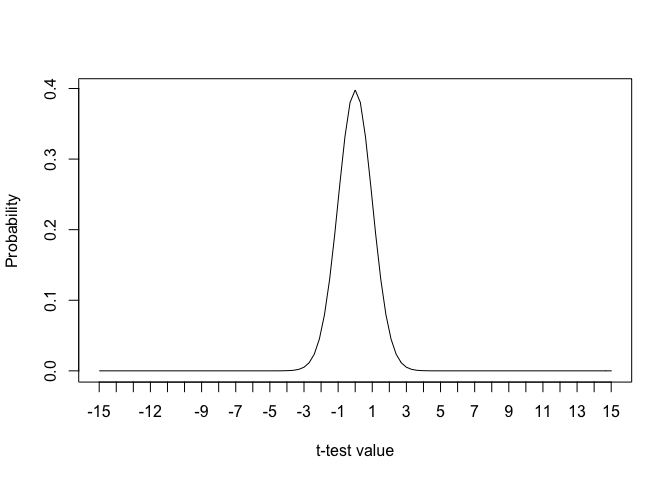
\includegraphics{img/unnamed-chunk-8-1.png}

The bell curve above illustrates all the possible \emph{t}-test results
one would expect when the null is true and their respective
probabilities. We see here that most results are within about +/- 3
points from zero. Where is our result? Let's add it to the plot.

\begin{figure}
\centering
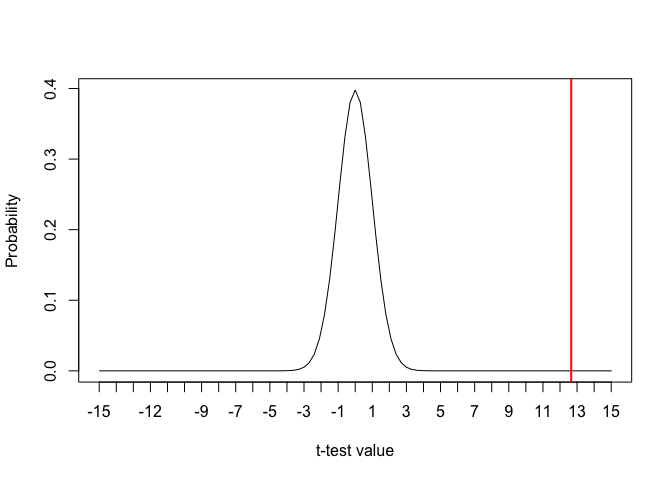
\includegraphics{img/unnamed-chunk-9-1.png}
\caption{}
\end{figure}

As we see, our result is out among values that are very, very rare under
the null hypothesis. It appears that our data disagree the null
hypothesis. When the null is true, we should be getting \emph{t}-test
results down in the center of the bell curve (approximately ± 3), but we
didn't. We were up at 10.8.

To find the \emph{p}-value, we simply ask what percentage of our
\emph{t}-curve is out that far. In other words, what proportion of the
bell curve extends out beyond the red line? What is the area "in the
upper tail"?

We can compute the p-value as \(1 - cdf\), for the t-statistic, where
\(cdf\) is the cumulative density function. The statsmodels
\texttt{t.cdf()} function computes the cdf given the t-statistic and the
degrees of freedom; \(n − 1 = 100 − 1 = 99\):

    \begin{Verbatim}[commandchars=\\\{\}]
{\color{incolor}In [{\color{incolor}7}]:} \PY{k+kn}{from} \PY{n+nn}{scipy}\PY{n+nn}{.}\PY{n+nn}{stats} \PY{k}{import} \PY{n}{t}
        \PY{l+m+mi}{1} \PY{o}{\PYZhy{}} \PY{n}{t}\PY{o}{.}\PY{n}{cdf}\PY{p}{(}\PY{l+m+mf}{10.8}\PY{p}{,} \PY{n}{df} \PY{o}{=} \PY{l+m+mi}{99}\PY{p}{,} \PY{n}{loc}\PY{o}{=}\PY{l+m+mi}{0}\PY{p}{,} \PY{n}{scale}\PY{o}{=}\PY{l+m+mi}{1}\PY{p}{)}
\end{Verbatim}


\begin{Verbatim}[commandchars=\\\{\}]
{\color{outcolor}Out[{\color{outcolor}7}]:} 0.0
\end{Verbatim}
            
    This result is saying there is "zero" probability of getting a result
this big if the null were true; i.e., \emph{p} = 0. In reality, \emph{p}
values are never zero but can get infinitely small. In this case the a
tiny number is rounded to 0.

This is called a on-tailed \emph{p}-value. We actually, however, need to
double it. The reason we need to double it is that our null hypothesis
was that \emph{μ} = 0. That is, the null is false if our result is
significantly \emph{larger} than zero (a positive attitude) or
significantly \emph{smaller} than zero (a negative attitude). This is
consistent with how we asked our question: "do people have positive or
negative attitudes?" In other words, we did not test a directional
prediction; we would be interested in "finding" something regardless of
the direction of the effect. Since the \emph{p}-value is the probability
of getting an effect "this large" and we do not care about the
direction, it actually exists on both sides of the distribution (a
negative attitude would have given us a negative \emph{t}-score):

\begin{figure}
\centering
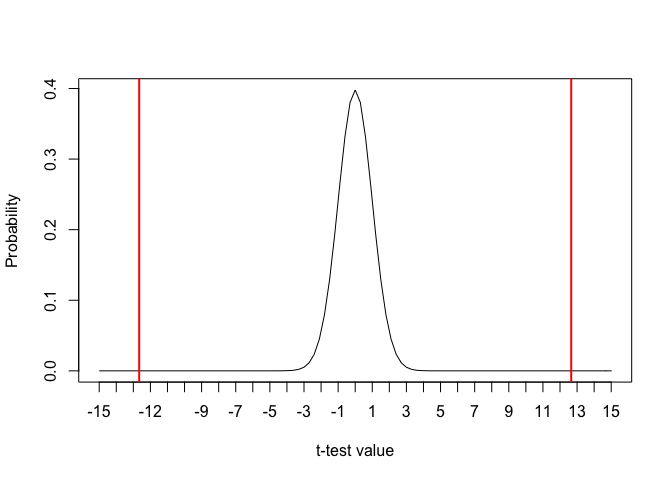
\includegraphics{img/unnamed-chunk-11-1.png}
\caption{}
\end{figure}

Thus, we have to double our \emph{p}-value. This is standard practice
any time you would be willing to declare the result significant
\textbf{regardless of the direction}. We call this a \emph{two-tailed
p-value}.

If this explanation is confusing, you can also understand it a slightly
different way: by testing \emph{H}0 : \emph{μ} = 0, you are really
asking whether \emph{μ} \textless{} 0 or whether
\emph{μ} \textgreater{} 0. You are essentially asking two separate
questions of the data. You need to double your \emph{p}-value.

This is almost always what you want. We almost always want to be able to
declare a result significant if the effect is large, regardless of
whether the direction of the result matches our intuition or not. For
example, if an intervention to increase productivity backfires and
decreases productivity, we want to know that just as much as we want to
know if it works.

Thus, we almost always double the \emph{p}-value for this reason. It is
true that it makes it a little harder to get a significant result (less
than .05), but we can extract more meaning from the result. It's worth
it.

Note: our doubled \emph{p}-value here is still essentially zero:

    \begin{Verbatim}[commandchars=\\\{\}]
{\color{incolor}In [{\color{incolor}8}]:} \PY{l+m+mf}{2.0} \PY{o}{*} \PY{p}{(}\PY{l+m+mi}{1} \PY{o}{\PYZhy{}} \PY{n}{t}\PY{o}{.}\PY{n}{cdf}\PY{p}{(}\PY{l+m+mf}{9.2}\PY{p}{,} \PY{l+m+mi}{100}\PY{p}{,} \PY{n}{loc}\PY{o}{=}\PY{l+m+mi}{0}\PY{p}{,} \PY{n}{scale}\PY{o}{=}\PY{l+m+mi}{1}\PY{p}{)}\PY{p}{)}
\end{Verbatim}


\begin{Verbatim}[commandchars=\\\{\}]
{\color{outcolor}Out[{\color{outcolor}8}]:} 5.551115123125783e-15
\end{Verbatim}
            

    % Add a bibliography block to the postdoc
    
    
    
    \end{document}
